\documentclass[11pt]{article}
\setlength{\topmargin}{0in}
\setlength{\headheight}{0in}
\setlength{\headsep}{0in}
\setlength{\textheight}{8.7in}
\setlength{\textwidth}{6.5in}
\setlength{\oddsidemargin}{0in}
\setlength{\evensidemargin}{0in}
\setlength{\parindent}{0.15in}
\setlength{\parskip}{0.05in}

\usepackage{graphics}

\begin{document}

\title{APC523: HW2 Problem 1}
\author{Miles Wu}
\maketitle

\section{Part a}
The following is true for any $i$-th row of $(T_\alpha \mathbf{q}_j)_i$ except for the first and last:
\begin{eqnarray*}
(T_\alpha \mathbf{q}_j)_i &=& - (\mathbf{q}_j)_{(i-1)} + \alpha (\mathbf{q}_j)_i - (\mathbf{q}_j)_{(i+1)} \\
&=&  - \sin ((i-1) j \theta) + \alpha \sin (i j \theta) - \sin ((i+1) j \theta) \\
&=& \alpha \sin (i j \theta) - \left(2 \sin(i j \theta) \cos(j \theta) - \cos(i j \theta) \sin(j \theta) + \cos(i j \theta) \sin(j \theta)\right)\\
&=& (\alpha - 2 \cos(j \theta)) \sin(i j \theta) \\
&=& (\lambda_j \mathbf{q}_j)_i
\end{eqnarray*}
For the first row we have:
\begin{eqnarray*}
(T_\alpha \mathbf{q}_j)_1 &=& \alpha (\mathbf{q}_j)_1 - (\mathbf{q}_j)_2 \\
&=&  \alpha \sin (j \theta) - \sin (2 j \theta) \\
&=& \alpha \sin (j \theta) - 2 \sin(j \theta) \cos (j \theta)\\
&=& (\alpha - 2 \cos(j \theta)) \sin(j \theta) \\
&=& (\lambda_j \mathbf{q}_j)_1
\end{eqnarray*}
For the last row we have: 
\begin{eqnarray*}
(T_\alpha \mathbf{q}_j)_n &=& \alpha (\mathbf{q}_j)_n - (\mathbf{q}_j)_{n-1} \\
&=&  \alpha \sin (n j \theta) - \sin ((n-1) j \theta) \\
\textnormal{because: } \sin ((n+1)j \theta) = \sin (j \pi) = 0
&=&  \alpha \sin (n j \theta) - \sin ((n-1) j \theta) - \sin ( (n+1) j \theta) \\
&=& \alpha \sin (n j \theta) - \left(2 \sin(n j \theta) \cos(j \theta) - \cos(n j \theta) \sin(j \theta) + \cos(n j \theta) \right)\\
&=& (\alpha - 2 \cos(j \theta)) \sin(n j \theta) \\
&=& (\lambda_j \mathbf{q}_j)_n
\end{eqnarray*}

Since $T_\alpha \mathbf{q}_j = \lambda_j \mathbf{q}_j$, $\lambda_j$ are the eigenvalues for the matrix and $\mathbf{q}_j$ are the corresponding eigenvectors.

For a matrix to be positive definite all the eigenvalues, $\lambda_j$, must be positive. For this to be true, $\alpha > -2 \cos (n \pi / (n+1))$.

\section{Part b}
This matrix is now identical to the one, except for an overall multiplicative factor of $1/h^2$, used in Section 2.2.3 for finite differences in a 1D second-derivative problem. 

\subsection{i}
The matrix is irreducibly diagonally dominant, because it is strictly diagonally dominant in the first and last row ($\alpha > |-1| $) and weakly diagonally dominant in the remaining rows ($\alpha \ge |-1| + |-1|$).

Yes; by Theorem 4.5, the Jacobi iterations will converge for any $x_0$, because the matrix is irreducibly diagonally dominant.

The Jacobi iteration matrix, $\mathbf{J}$ is:
\begin{eqnarray*}
\mathbf{J} &=& -\mathbf{D}^{-1} ( \mathbf{L} + \mathbf{U}) \\
&=& \frac{-1}{\alpha} \mathbf{I} ( \mathbf{L} + \mathbf{U}) \\
&=& \frac{-1}{\alpha}
\left( \begin{array}{cccc}
0 & -1 & 0 & 0 \\
-1 & 0 & -1 & 0 \\
0 & -1 & 0 & -1 \\
0 & 0 & -1 & 0
\end{array} \right)
\end{eqnarray*}
This is the same as matrix $\mathbf{T}_{0}$ where $\alpha = 0$. Therefore the eigenvalues of $\mathbf{J}$ are: $\lambda_j = - 2/\alpha \cos (j \theta) $, where $\alpha = 2$. The convergence factor is therefore:
\begin{eqnarray*}
\rho &=& \rho(\mathbf{J}) = \textnormal{max} |\lambda_j| \\
&=& \cos \theta
\end{eqnarray*}

\subsection{ii}
Yes; by Theorem 4.5, the Gauss-Seidel iterations will converge for any $x_0$, because the matrix is irreducibly diagonally dominant.
If we take $\omega = 1$, we see that the SOR matrix is the same as the Gauss-Seidel iteration matrix, $\mathbf{G}$:

\begin{eqnarray*}
\mathbf{M}_{SOR} &=& (\mathbf{D} - \omega \mathbf{E})^{-1} (\omega \mathbf{F} + (1-\omega) \mathbf{D}) \\
&=& (\mathbf{D} - \mathbf{E})^{-1} \mathbf{F} \\
&=& \mathbf{G}
\end{eqnarray*}

By Theorem 4.7, we have $(\lambda_{SOR} + \omega - 1)^2 = \lambda_{SOR} \omega^2 \lambda_J^2$, where $\lambda_J$ are the eigenvalues of the Jacobi iteration matrix dervied in the earlier question. With $\omega = 1$, we find that the eigenvalues of the SOR iteration matrix are the square of the eigenvalues of the Jacobi iteration matrix, $\mathbf{J}$. Therefore the convergence factor is:
\begin{eqnarray*}
\rho &=& \rho(\mathbf{G}) = \rho(\mathbf{M_{SOR}}) \\
&=& \textnormal{max} |\lambda_j|^2 \\
&=& \cos^2 \theta
\end{eqnarray*}


\subsection{iii}
By Theorem 4.6, the SOR iterations will converge for $0 \le \omega \le 2$ for any $x_0$, because the matrix is symmetric with positive diagonal elements and is positive definite.

\section{Part c}
Since $\rho_G = {\rho_J}^2$ as proven in the earlier questions, for every iteration of Gauss-Seidel we must do two iterations of Jacobi. Therefore we need twice as many iterations of Jacobi to achieve the same error as Gauss-Seidel.

\section{Part d}

\begin{figure}
\begin{center}
% GNUPLOT: LaTeX picture with Postscript
\begingroup
  \makeatletter
  \providecommand\color[2][]{%
    \GenericError{(gnuplot) \space\space\space\@spaces}{%
      Package color not loaded in conjunction with
      terminal option `colourtext'%
    }{See the gnuplot documentation for explanation.%
    }{Either use 'blacktext' in gnuplot or load the package
      color.sty in LaTeX.}%
    \renewcommand\color[2][]{}%
  }%
  \providecommand\includegraphics[2][]{%
    \GenericError{(gnuplot) \space\space\space\@spaces}{%
      Package graphicx or graphics not loaded%
    }{See the gnuplot documentation for explanation.%
    }{The gnuplot epslatex terminal needs graphicx.sty or graphics.sty.}%
    \renewcommand\includegraphics[2][]{}%
  }%
  \providecommand\rotatebox[2]{#2}%
  \@ifundefined{ifGPcolor}{%
    \newif\ifGPcolor
    \GPcolorfalse
  }{}%
  \@ifundefined{ifGPblacktext}{%
    \newif\ifGPblacktext
    \GPblacktexttrue
  }{}%
  % define a \g@addto@macro without @ in the name:
  \let\gplgaddtomacro\g@addto@macro
  % define empty templates for all commands taking text:
  \gdef\gplbacktext{}%
  \gdef\gplfronttext{}%
  \makeatother
  \ifGPblacktext
    % no textcolor at all
    \def\colorrgb#1{}%
    \def\colorgray#1{}%
  \else
    % gray or color?
    \ifGPcolor
      \def\colorrgb#1{\color[rgb]{#1}}%
      \def\colorgray#1{\color[gray]{#1}}%
      \expandafter\def\csname LTw\endcsname{\color{white}}%
      \expandafter\def\csname LTb\endcsname{\color{black}}%
      \expandafter\def\csname LTa\endcsname{\color{black}}%
      \expandafter\def\csname LT0\endcsname{\color[rgb]{1,0,0}}%
      \expandafter\def\csname LT1\endcsname{\color[rgb]{0,1,0}}%
      \expandafter\def\csname LT2\endcsname{\color[rgb]{0,0,1}}%
      \expandafter\def\csname LT3\endcsname{\color[rgb]{1,0,1}}%
      \expandafter\def\csname LT4\endcsname{\color[rgb]{0,1,1}}%
      \expandafter\def\csname LT5\endcsname{\color[rgb]{1,1,0}}%
      \expandafter\def\csname LT6\endcsname{\color[rgb]{0,0,0}}%
      \expandafter\def\csname LT7\endcsname{\color[rgb]{1,0.3,0}}%
      \expandafter\def\csname LT8\endcsname{\color[rgb]{0.5,0.5,0.5}}%
    \else
      % gray
      \def\colorrgb#1{\color{black}}%
      \def\colorgray#1{\color[gray]{#1}}%
      \expandafter\def\csname LTw\endcsname{\color{white}}%
      \expandafter\def\csname LTb\endcsname{\color{black}}%
      \expandafter\def\csname LTa\endcsname{\color{black}}%
      \expandafter\def\csname LT0\endcsname{\color{black}}%
      \expandafter\def\csname LT1\endcsname{\color{black}}%
      \expandafter\def\csname LT2\endcsname{\color{black}}%
      \expandafter\def\csname LT3\endcsname{\color{black}}%
      \expandafter\def\csname LT4\endcsname{\color{black}}%
      \expandafter\def\csname LT5\endcsname{\color{black}}%
      \expandafter\def\csname LT6\endcsname{\color{black}}%
      \expandafter\def\csname LT7\endcsname{\color{black}}%
      \expandafter\def\csname LT8\endcsname{\color{black}}%
    \fi
  \fi
  \setlength{\unitlength}{0.0500bp}%
  \begin{picture}(7200.00,5040.00)%
    \gplgaddtomacro\gplbacktext{%
      \csname LTb\endcsname%
      \put(1342,704){\makebox(0,0)[r]{\strut{} 0.0001}}%
      \put(1342,2061){\makebox(0,0)[r]{\strut{} 0.001}}%
      \put(1342,3418){\makebox(0,0)[r]{\strut{} 0.01}}%
      \put(1342,4775){\makebox(0,0)[r]{\strut{} 0.1}}%
      \put(1474,484){\makebox(0,0){\strut{} 0}}%
      \put(2007,484){\makebox(0,0){\strut{} 1000}}%
      \put(2540,484){\makebox(0,0){\strut{} 2000}}%
      \put(3073,484){\makebox(0,0){\strut{} 3000}}%
      \put(3606,484){\makebox(0,0){\strut{} 4000}}%
      \put(4139,484){\makebox(0,0){\strut{} 5000}}%
      \put(4671,484){\makebox(0,0){\strut{} 6000}}%
      \put(5204,484){\makebox(0,0){\strut{} 7000}}%
      \put(5737,484){\makebox(0,0){\strut{} 8000}}%
      \put(6270,484){\makebox(0,0){\strut{} 9000}}%
      \put(6803,484){\makebox(0,0){\strut{} 10000}}%
      \put(176,2739){\rotatebox{-270}{\makebox(0,0){\strut{}Error}}}%
      \put(4138,154){\makebox(0,0){\strut{}Number of iterations}}%
      \put(3073,4065){\makebox(0,0)[l]{\strut{}Fit to $A \rho^x$: $\rho = 0.999516 \pm 5 \times 10^{-12}$}}%
    }%
    \gplgaddtomacro\gplfronttext{%
    }%
    \gplbacktext
    \put(0,0){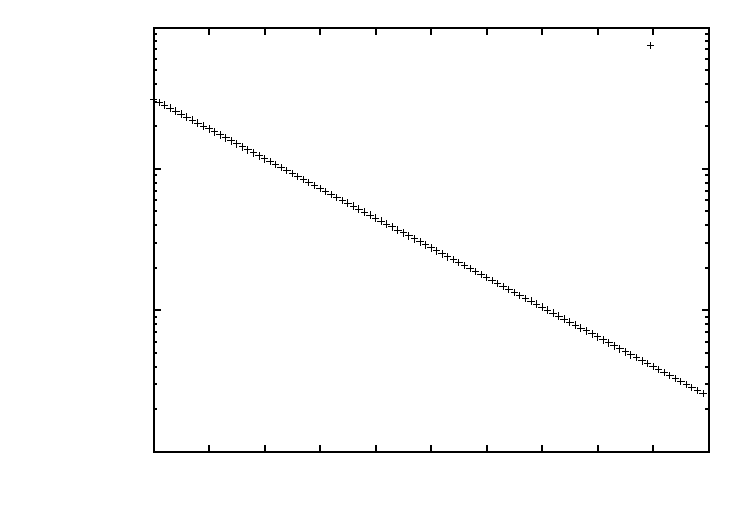
\includegraphics{jacobi_j_1}}%
    \gplfronttext
  \end{picture}%
\endgroup

\caption{ A plot showing the error as a function of the number of iterations for $j=1$. The $y$ axis is a log scale. A best fit line to the function form of $A p^x$ was also calculated, where $\rho$ is the convergence factor, and this parameter labeled on the plot.  }
\label{j1}
\end{center}
\end{figure}

\begin{figure}
\begin{center}
% GNUPLOT: LaTeX picture with Postscript
\begingroup
  \makeatletter
  \providecommand\color[2][]{%
    \GenericError{(gnuplot) \space\space\space\@spaces}{%
      Package color not loaded in conjunction with
      terminal option `colourtext'%
    }{See the gnuplot documentation for explanation.%
    }{Either use 'blacktext' in gnuplot or load the package
      color.sty in LaTeX.}%
    \renewcommand\color[2][]{}%
  }%
  \providecommand\includegraphics[2][]{%
    \GenericError{(gnuplot) \space\space\space\@spaces}{%
      Package graphicx or graphics not loaded%
    }{See the gnuplot documentation for explanation.%
    }{The gnuplot epslatex terminal needs graphicx.sty or graphics.sty.}%
    \renewcommand\includegraphics[2][]{}%
  }%
  \providecommand\rotatebox[2]{#2}%
  \@ifundefined{ifGPcolor}{%
    \newif\ifGPcolor
    \GPcolorfalse
  }{}%
  \@ifundefined{ifGPblacktext}{%
    \newif\ifGPblacktext
    \GPblacktexttrue
  }{}%
  % define a \g@addto@macro without @ in the name:
  \let\gplgaddtomacro\g@addto@macro
  % define empty templates for all commands taking text:
  \gdef\gplbacktext{}%
  \gdef\gplfronttext{}%
  \makeatother
  \ifGPblacktext
    % no textcolor at all
    \def\colorrgb#1{}%
    \def\colorgray#1{}%
  \else
    % gray or color?
    \ifGPcolor
      \def\colorrgb#1{\color[rgb]{#1}}%
      \def\colorgray#1{\color[gray]{#1}}%
      \expandafter\def\csname LTw\endcsname{\color{white}}%
      \expandafter\def\csname LTb\endcsname{\color{black}}%
      \expandafter\def\csname LTa\endcsname{\color{black}}%
      \expandafter\def\csname LT0\endcsname{\color[rgb]{1,0,0}}%
      \expandafter\def\csname LT1\endcsname{\color[rgb]{0,1,0}}%
      \expandafter\def\csname LT2\endcsname{\color[rgb]{0,0,1}}%
      \expandafter\def\csname LT3\endcsname{\color[rgb]{1,0,1}}%
      \expandafter\def\csname LT4\endcsname{\color[rgb]{0,1,1}}%
      \expandafter\def\csname LT5\endcsname{\color[rgb]{1,1,0}}%
      \expandafter\def\csname LT6\endcsname{\color[rgb]{0,0,0}}%
      \expandafter\def\csname LT7\endcsname{\color[rgb]{1,0.3,0}}%
      \expandafter\def\csname LT8\endcsname{\color[rgb]{0.5,0.5,0.5}}%
    \else
      % gray
      \def\colorrgb#1{\color{black}}%
      \def\colorgray#1{\color[gray]{#1}}%
      \expandafter\def\csname LTw\endcsname{\color{white}}%
      \expandafter\def\csname LTb\endcsname{\color{black}}%
      \expandafter\def\csname LTa\endcsname{\color{black}}%
      \expandafter\def\csname LT0\endcsname{\color{black}}%
      \expandafter\def\csname LT1\endcsname{\color{black}}%
      \expandafter\def\csname LT2\endcsname{\color{black}}%
      \expandafter\def\csname LT3\endcsname{\color{black}}%
      \expandafter\def\csname LT4\endcsname{\color{black}}%
      \expandafter\def\csname LT5\endcsname{\color{black}}%
      \expandafter\def\csname LT6\endcsname{\color{black}}%
      \expandafter\def\csname LT7\endcsname{\color{black}}%
      \expandafter\def\csname LT8\endcsname{\color{black}}%
    \fi
  \fi
  \setlength{\unitlength}{0.0500bp}%
  \begin{picture}(7200.00,5040.00)%
    \gplgaddtomacro\gplbacktext{%
      \csname LTb\endcsname%
      \put(1342,704){\makebox(0,0)[r]{\strut{} 1e-11}}%
      \put(1342,1111){\makebox(0,0)[r]{\strut{} 1e-10}}%
      \put(1342,1518){\makebox(0,0)[r]{\strut{} 1e-09}}%
      \put(1342,1925){\makebox(0,0)[r]{\strut{} 1e-08}}%
      \put(1342,2332){\makebox(0,0)[r]{\strut{} 1e-07}}%
      \put(1342,2740){\makebox(0,0)[r]{\strut{} 1e-06}}%
      \put(1342,3147){\makebox(0,0)[r]{\strut{} 1e-05}}%
      \put(1342,3554){\makebox(0,0)[r]{\strut{} 0.0001}}%
      \put(1342,3961){\makebox(0,0)[r]{\strut{} 0.001}}%
      \put(1342,4368){\makebox(0,0)[r]{\strut{} 0.01}}%
      \put(1342,4775){\makebox(0,0)[r]{\strut{} 0.1}}%
      \put(1474,484){\makebox(0,0){\strut{} 0}}%
      \put(2007,484){\makebox(0,0){\strut{} 1000}}%
      \put(2540,484){\makebox(0,0){\strut{} 2000}}%
      \put(3073,484){\makebox(0,0){\strut{} 3000}}%
      \put(3606,484){\makebox(0,0){\strut{} 4000}}%
      \put(4139,484){\makebox(0,0){\strut{} 5000}}%
      \put(4671,484){\makebox(0,0){\strut{} 6000}}%
      \put(5204,484){\makebox(0,0){\strut{} 7000}}%
      \put(5737,484){\makebox(0,0){\strut{} 8000}}%
      \put(6270,484){\makebox(0,0){\strut{} 9000}}%
      \put(6803,484){\makebox(0,0){\strut{} 10000}}%
      \put(176,2739){\rotatebox{-270}{\makebox(0,0){\strut{}Error}}}%
      \put(4138,154){\makebox(0,0){\strut{}Number of iterations}}%
      \put(3073,4562){\makebox(0,0)[l]{\strut{}Fit to $A \rho^x$: $\rho = 0.998066 \pm 2\times 10^{-10}$}}%
    }%
    \gplgaddtomacro\gplfronttext{%
    }%
    \gplbacktext
    \put(0,0){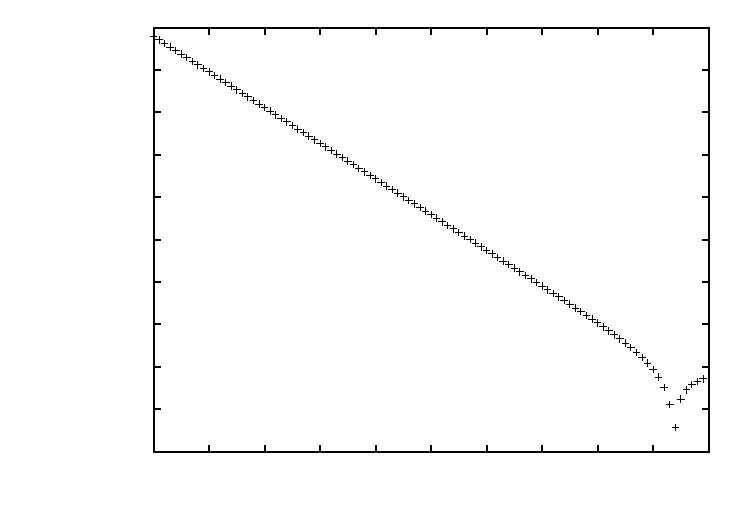
\includegraphics{jacobi_j_2}}%
    \gplfronttext
  \end{picture}%
\endgroup

\caption{ A plot showing the error as a function of the number of iterations for $j=2$. The $y$ axis is a log scale. A best fit line to the function form of $A p^x$ was also calculated, where $\rho$ is the convergence factor, and this parameter labeled on the plot.  }
\label{j2}
\end{center}
\end{figure}

\subsection{i}
Figure \ref{j1} is the plot showing the error as a function of the number of iterations.

The convergence factor is indeed $\rho(G_J)$ in this case, because we are solving for the dominant eigenvalue which is the same one as the general convergence factor and the spectral radius. This is shown in the fit to the data where $\rho = 0.999516$. This matches with $\rho(G_J) = \cos (\pi/101) = 0.999516$. 

\subsection{ii}
Figure \ref{j2} is the plot showing the error as a function of the number of iterations. The weird behaviour around 9000 iterations is due to the limits of double precision on computers and we can safely ignore that section of the plot.

The convergence factor is not $\rho(G_J)$ in this case, because we are solving for an $x$ that does not contain a component corresponding to the dominant eigenvalue. This is shown in the fit to the data where $\rho = 0.998066$, which does not match with $\rho(G_J) = \cos (\pi/101) = 0.999516$.

The analytical expression for the convergence factor is: $\rho_j = \cos( j \pi / 101)$. For example, $\rho_2 = 0.998065597$ which corresponds with our fit.
\subsection{iii}
If $x$ is a linear combination of the eigenvectors, $q_j$, then the error would behave in a more complex way. The error for each component of the linear combination would decay according to each eigenvector's convergence factor. This would lead initially to a faster decay (as the error components that aren't the dominant eigenvalue would decay much quicker), but after a while it will slow down to the usual global convergence factor (as all the non-dominant eigenvalue error components are already pretty much 0 by this point leaving only the dominant one).

$\rho(G_J)$ is not an accurate estimator of the convergence rate when $k$ is small, because as mentioned above the error initially decays faster due to the non-dominant eigenvalue error components. However, as $k$ tends to infinity, it becomes a more accurate estimator, the most significant error left is the dominant one and this goes like $\rho(G_J)$.


\end{document}